\chapter{Background}

\section{Overview}

<block diagram of vehicle systems>

\section{Transmission}


\subsection{Overview}

Brief {}``what is transmission''

Shifting speed and dexterity required

Stall avoidance

-one chance to restart during race

-sensitivity to stalling

launching the car, etc.


\subsection{Mechanical Systems}

Simple descriptions


\subsubsection{Clutch}


\subsubsection{Gear Selection}


\subsection{Previous Implementations and Shortcomings}

How, challenges, etc.


\subsubsection{Electropneumatic Actuation}


\subsubsection{Gear Position Sensing}


\subsubsection{Neutral Sensing}


\section{Engine}


\subsection{Overview}

brief {}``what is engine'', honda cbr, etc.

maximise power output (performance application)

torque power curve, etc.


\subsection{Intake and Exhaust}

Intake background, pressure waves, etc. Torque curve depends on length, 


\subsection{Research and Modelling of Variable Length Intake}

present research done by others on team, quantified runner length
dependence

intake length changes power

quantified length versus power on actual vehicle

chose optimal intake length

proposed variable length intake system for future work


\subsection{Starting System}

current requirements, starter motor, etc.


\section{Braking}


\subsection{Overview}

Idea of braking and force distribution


\subsection{Mechanical Systems}


\subsubsection{Independant Hydraulic Systems}


\subsubsection{Balance Bar}


\subsection{Adjustment Difficulties}

Competition problems, manual adjustment difficulty, scope of adjustment,
tuneability lag

\section{Pre-existing Off-the-shelf Modules}

There are two off-the-shelf electronic modules as part of the pre-existing equipment on the car, the ECU and the DAC.

\subsection{ECU}

A specialized third-party component called the \emph{Engine Control Unit} (ECU) controls the fuel injector and spark coil systems that in turn control the combustion cycle of the engine. The particular model of ECU used by the Formula SAE car is the S80Pro from DTAFast \cite{s80pro}. The ECU uses the O$_{2}$, MAP, cam position, and crank position sensors to adjust the fuel injector and spark coil timings. This keeps the engine running smoothly. The ECU features a traction control system that monitors wheel slip and cuts spark and fuel to provide traction when one of the wheels is slipping. The ECU also collects the various sensor readings and makes them available to other electronic devices at a fixed frequency through a shared data bus. 

\begin{figure}[H]
\centering
%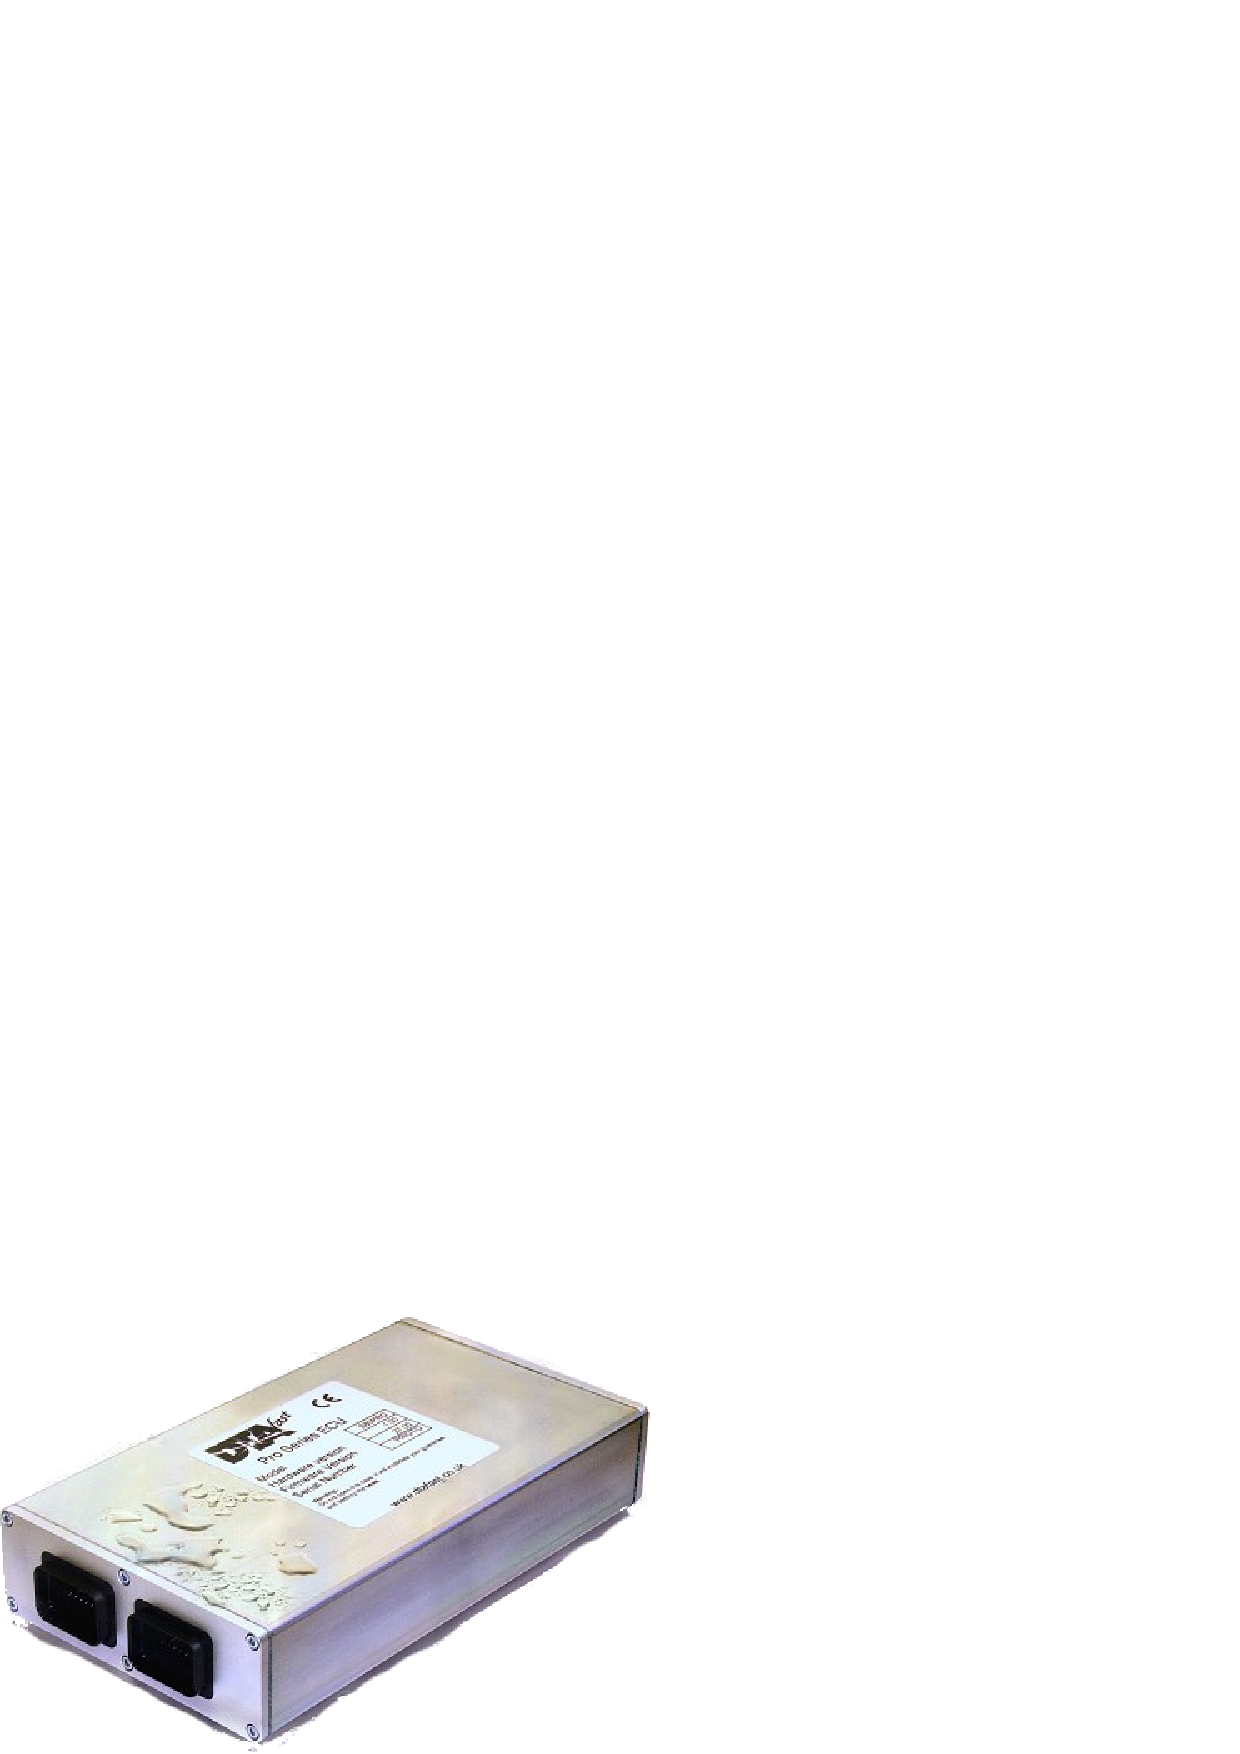
\includegraphics[scale=0.5]{Figures/s80.png}
\caption{The DTAFast S80Pro engine control unit.}
\label{fig:s80pro_product}
\end{figure}

\subsubsection{ECU Data interfaces\label{sec:background_ecu_data_interfaces}}

The ECU provides 3 digital communication methods:
\begin{itemize}
  \item An RS-232 link is used by the software that DTA provides for tuning and controlling the ECU. The serial protocol that the software uses is proprietary and undocumented.
  \item A read-only CAN bus interface that emits ECU data at a fixed frequency. The message format for the CAN data is documented in Appendix \ref{cha:ecu_can_spec}.
  \item Several CMOS-level discrete inputs:
  \begin{itemize}
    \item Launch Control toggle, which toggles the launch control feature in the ECU,
    \item Shift cut, which signals the ECU to reduce engine power before a downshift
    \item Traction control toggle, which toggles the traction control feature in the ECU,
    \item Traction control wet/dry, which switches between two different sets of traction control parameters in the ECU.
  \end{itemize}
\end{itemize}

Detailed descriptions of the ECU's launch control, shift cut, and traction control features can be found in the manual \cite{s80pro}.
 
\nomenclature{RS-232}{Recommended Standard 232, a byte-oriented serial communications protocol, typically asynchronous.}

\subsection{DAC}

Another specialized third-party component called the \emph{Data Acquisition Device} (DAC) is used to log and relay sensor data to other electronic devices.

The particular DAC used is the model DL1 from Race Technology \cite{DL1Dsheet}. The DL1 is an expandable data logger with built-in 20-Hz GPS and 3-axis accelerometer.

\subsubsection{DAC Data Interface\label{sec:background_dac_data_interface}}

Race Technology provides a software suite that communicates with the DAC using a documented serial protocol. Every item that the DAC logs is output to its own channel in real time on the serial port. It is also possible to configure the software to recognize new channels for arbitrary types of data.

\begin{figure}[H]
\centering
%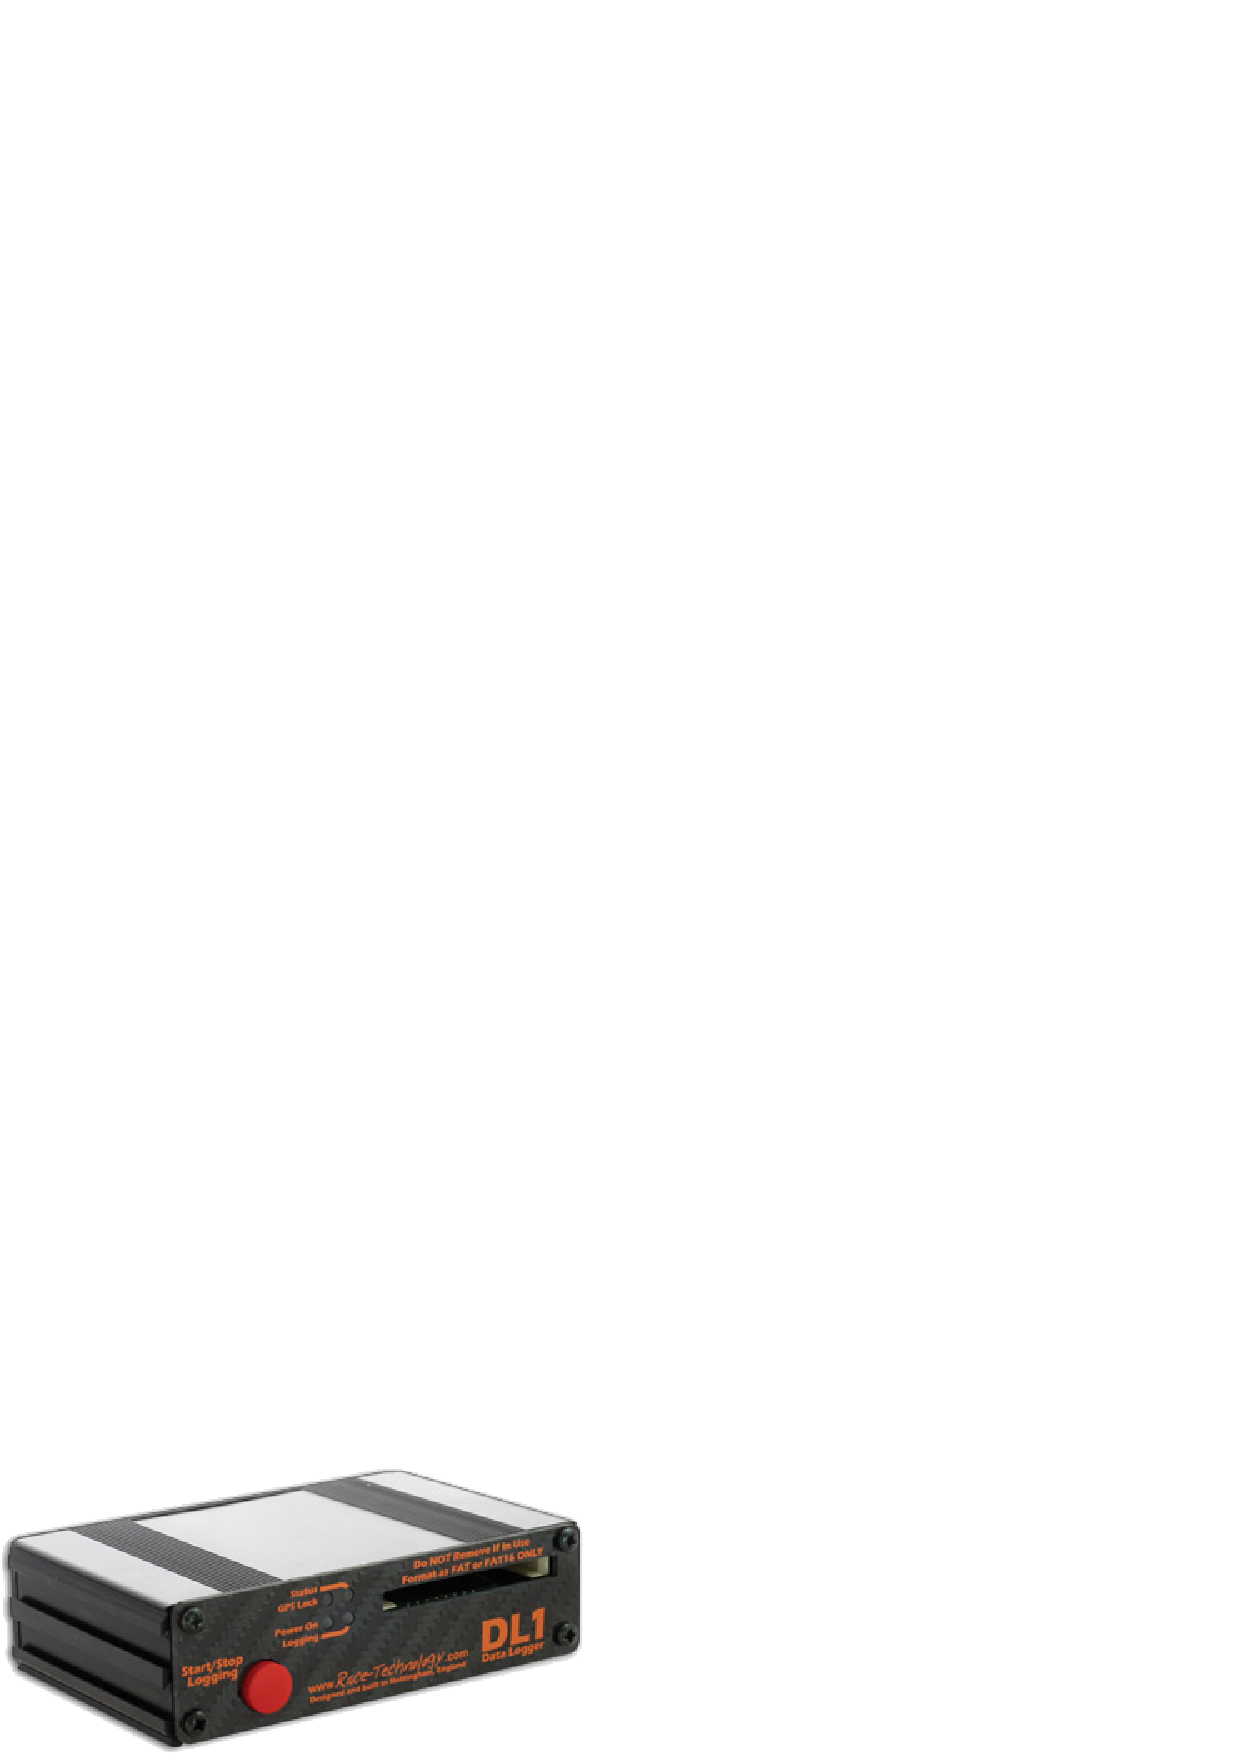
\includegraphics[scale=0.5]{Figures/dl1.png}
\caption{The Race Systems DL1 data acquisition device.}
\label{fig:dl1_product}
\end{figure}


\section{Telemetry}

\subsection{Overview}

The manufacturers of both the ECU and the DAC provide specialized PC software that communicates with the modules using the serial data interfaces described above. The intended procedure for using these interfaces is by physically connecting a hard serial cable from the modules to a PC running the software. This however limits mobility, and requires the plugging and unplugging of cables.

Why is telemetry necessary? Sensors, data, etc.

\subsection{Previous Implementations and Shortcomings}


\subsubsection{Cellular Link}


\subsubsection{Off-the-Shelf XBee Link}

Both of these only worked with one device, weren't reliable, etc.


\section{Driver Interface}


\subsection{Overview}

Driver and crew needs easy access to data, easy control of on-board
systems


\subsection{Driver Controls}


\subsubsection{Transmission Control}

Upshift/Downshift

Activate other trans. control features, neutral find, etc., launch


\subsubsection{Engine Control}


\subsection{Vehicle Diagnostics}


\subsubsection{Critical Indicators}

Overheating, oil pressure, etc.


\subsubsection{Supplimentary Indicators}

information about telemetry, shift control, etc.


\subsection{Previous Implementations and Shortcomings}